\documentclass{article}
\usepackage[paperwidth=190mm,paperheight=100mm,margin=4mm]{geometry}
\usepackage{xcolor}
\usepackage{tikz}
\usetikzlibrary{arrows.meta,backgrounds,fit,positioning,shapes.geometric}
\pagestyle{empty}

\definecolor{PremiumEmerald}{HTML}{064E3B}
\definecolor{Emerald}{HTML}{047857}
\definecolor{EmeraldMist}{HTML}{EAF5F0}
\definecolor{EmeraldWash}{HTML}{F5FAF7}
\definecolor{Charcoal}{HTML}{17211D}
\definecolor{MutedInk}{HTML}{52605A}
\definecolor{SoftRule}{HTML}{C8D9D1}

\begin{document}
\centering
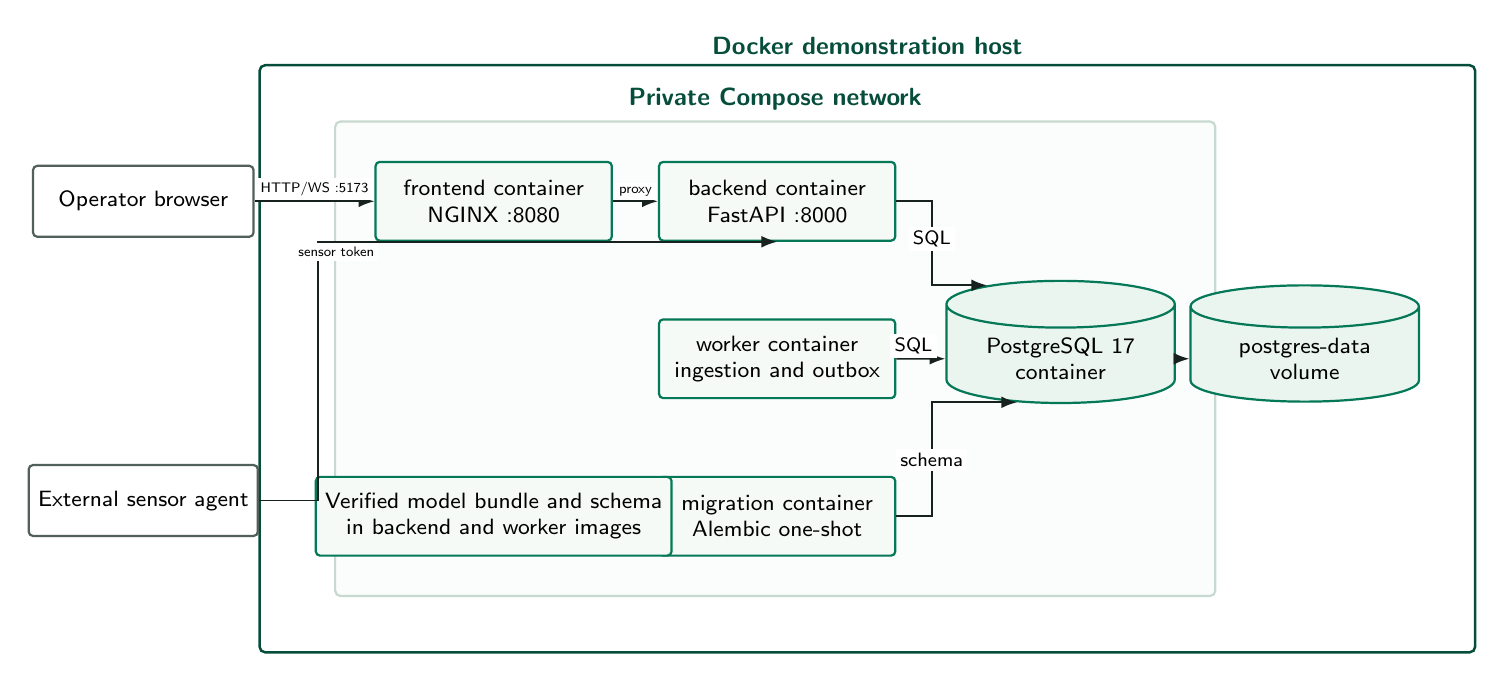
\begin{tikzpicture}[
  font=\sffamily\footnotesize,
  container/.style={draw=Emerald,fill=EmeraldWash,rounded corners=1.5pt,
    minimum width=30mm,minimum height=10mm,align=center,line width=.8pt},
  external/.style={draw=MutedInk,fill=white,rounded corners=1.5pt,
    minimum width=28mm,minimum height=9mm,align=center,line width=.8pt},
  store/.style={draw=Emerald,fill=EmeraldMist,cylinder,shape border rotate=90,
    aspect=.28,minimum width=29mm,minimum height=12mm,align=center,line width=.8pt},
  boundary/.style={draw=SoftRule,fill=EmeraldWash!45,rounded corners=2pt,
    inner sep=5mm,line width=.8pt},
  host/.style={draw=PremiumEmerald,fill=none,rounded corners=2pt,
    inner sep=7mm,line width=.9pt},
  flow/.style={-{Latex[length=2mm]},draw=Charcoal,line width=.7pt},
  package/.style={-{Latex[length=2mm]},draw=MutedInk,dashed,line width=.65pt},
  edge/.style={font=\sffamily\scriptsize,fill=white,inner sep=1.5pt,align=center}
]
  \node[external] (browser) at (-7.1,2.15) {Operator browser};
  \node[external] (sensor) at (-7.1,-1.65) {External sensor agent};

  \node[container] (frontend) at (-2.65,2.15) {frontend container\\NGINX :8080};
  \node[container] (backend) at (0.95,2.15) {backend container\\FastAPI :8000};
  \node[container] (worker) at (0.95,0.15) {worker container\\ingestion and outbox};
  \node[container] (migration) at (0.95,-1.85) {migration container\\Alembic one-shot};
  \node[store] (database) at (4.55,0.15) {PostgreSQL 17\\container};
  \node[store] (volume) at (7.65,0.15) {postgres-data\\volume};
  \node[container] (bundle) at (-2.65,-1.85) {Verified model bundle and schema\\in backend and worker images};

  \begin{scope}[on background layer]
    \node[boundary,fit=(frontend)(backend)(worker)(migration)(database),
      label={[font=\sffamily\bfseries\small\color{PremiumEmerald}]above:Private Compose network}] (network) {};
    \node[host,fit=(network)(volume)(bundle),
      label={[font=\sffamily\bfseries\small\color{PremiumEmerald}]above:Docker demonstration host}] {};
  \end{scope}

  \draw[flow] (browser.east) -- node[edge,above,font=\sffamily\tiny] {HTTP/WS :5173} (frontend.west);
  \draw[flow] (sensor.east) -- ++(.75,0) |- node[edge,pos=.52,below,font=\sffamily\tiny] {sensor token} (backend.south);
  \draw[flow] (frontend) -- node[edge,above,font=\sffamily\tiny] {proxy} (backend);
  \draw[flow] (backend.east) -- ++(.45,0) |- node[edge,pos=.30,above] {SQL} (database.north west);
  \draw[flow] (worker) -- node[edge,above,pos=.35] {SQL} (database);
  \draw[flow] (migration.east) -- ++(.45,0) |- node[edge,pos=.30,below] {schema} (database.south west);
  \draw[flow] (database) -- (volume);
\end{tikzpicture}
\end{document}
